\documentclass[aspectratio=169,notes]{beamer}
\usepackage{lmodern}
\usepackage[T1]{fontenc}
\usepackage{textcomp}
\usepackage{animate}
\usepackage{underscore}
\usepackage{pdfpc-commands}
\usepackage{xmpmulti}
\usepackage{multimedia}
\usepackage{epstopdf}
\usepackage{bbding}
\usepackage{hyperref}
\usepackage{listings}
\lstdefinelanguage{D}
{
  % list of keywords
  morekeywords={
abstract,
alias,
align,
asm,
assert,
auto,
body,
bool,
break,
byte,
case,
cast,
catch,
cdouble,
cent,
cfloat,
char,
class,
const,
continue,
creal,
dchar,
debug,
default,
delegate,
delete (deprecated),
deprecated,
do,
double,
else,
enum,
export,
extern,
false,
final,
finally,
float,
for,
foreach,
foreach_reverse,
function,
goto,
idouble,
if,
ifloat,
immutable,
import,
in,
inout,
int,
interface,
invariant,
ireal,
is,
lazy,
long,
mixin,
module,
new,
nothrow,
null,
out,
override,
package,
pragma,
private,
protected,
public,
pure,
real,
ref,
return,
scope,
shared,
short,
static,
string,
struct,
super,
switch,
synchronized,
template,
this,
throw,
true,
try,
typeid,
typeof,
ubyte,
ucent,
uint,
ulong,
union,
unittest,
ushort,
version,
void,
wchar,
while,
with,
__FILE__,
__FILE_FULL_PATH__,
__MODULE__,
__LINE__,
__FUNCTION__,
__PRETTY_FUNCTION__,
__gshared,
__traits,
__vector,
__parameters
  },
  sensitive=false, % keywords are not case-sensitive
  morecomment=[l]{//}, % l is for line comment
  morecomment=[s]{/*}{*/}, % s is for start and end delimiter
  morecomment=[s]{/+}{+/}, % s is for start and end delimiter
  morestring=[b]" % defines that strings are enclosed in double quotes
}
\usepackage{color}
\definecolor{eclipseBlue}{RGB}{42,0.0,255}
\definecolor{eclipseGreen}{RGB}{63,127,95}
\definecolor{eclipsePurple}{RGB}{127,0,85}
 
% Set Language
\lstset{
  language={D},
  basicstyle=\small\ttfamily, % Global Code Style
  captionpos=b, % Position of the Caption (t for top, b for bottom)
  extendedchars=true, % Allows 256 instead of 128 ASCII characters
  tabsize=2, % number of spaces indented when discovering a tab 
  columns=fixed, % make all characters equal width
  keepspaces=true, % does not ignore spaces to fit width, convert tabs to spaces
  showstringspaces=false, % lets spaces in strings appear as real spaces
  breaklines=true, % wrap lines if they don't fit
  numbers=left, % show line numbers at the left
  numberstyle=\tiny\ttfamily, % style of the line numbers
  commentstyle=\color{eclipseGreen}, % style of comments
  keywordstyle=\color{eclipsePurple}, % style of keywords
  stringstyle=\color{eclipseBlue}, % style of strings
}
\usepackage{tikz}
\usetikzlibrary{shadows}
\usepackage{xkeyval}
\usepackage{todonotes}
\presetkeys{todonotes}{inline}{}
\defbeamertemplate{description item}{align left}{\insertdescriptionitem\hfill}
\usetheme{metropolis}					 % Use metropolis theme
\usepackage[
    backend=biber,
    url=true, 
	style=numeric,
    doi=true,
    eprint=false
]{biblatex}
\addbibresource{biblatex-examples.bib}

\title{All Spreadsheets must Die}
\date{\today}
\author{Robert Schadek}
\begin{document}
	\maketitle

	\section{Getting started}
	\begin{frame}{A random list of languages we love to hate}
		\begin{itemize}
			\item Rust
			\item Go
			\item C++
			\item JavaScript
			\item Typescript
		\end{itemize}
		\todo{replace itemize with logos}
	\end{frame}

	\note[itemize]{
		\item There are all these languages we like to hate.
		\item Many of them are good, many are more popular.
		\item Many might even be better.
		\item But we are missing something
	}

	\begin{frame}{Hating by numbers}
		\begin{description}
			\item[C++] $4.4 Million$ (2015)
			\item[C] $1.9 Million$ (2015)
			\item[Java] $9 Million$ (2009)	
			\item[JS] $10 Million$ (2018)
		\end{description}
	\end{frame}
	
	\begin{frame}
		\begin{center}
		\huge
		These are all small fish\\[2cm]
		\pause
		\textbf{Excel} $750 Million$ (2016)
		\end{center}
	\end{frame}

	\begin{frame}[fragile]
		\begin{center}
		\includegraphics[width=0.6\textwidth]{skepical.jpg}
		\end{center}
	\end{frame}

	\begin{frame}[fragile]{Oh, but it is \hfill{} \cite{GOTO201638:online}}
		\begin{center}
		\includegraphics[width=1.0\textwidth]{functionalexcel.jpg}
		\end{center}
	\end{frame}

	\section{A little bit of Spreadsheet bashing}
	\begin{frame}[fragile]{See the code is difficult}
		\begin{center}
		\includegraphics[width=1.0\textwidth]{excelseeingcode.jpg}
		\end{center}
	\end{frame}

	\begin{frame}[fragile]{Dynamic Types}
		\begin{center}
		\includegraphics[width=1.0\textwidth]{exceldynamic.jpg}
		\end{center}
	\end{frame}

	\begin{frame}[fragile]{Dynamic Types}
		\begin{center}
		\includegraphics[width=1.0\textwidth]{exceldynamic2.jpg}
		\end{center}
	\end{frame}

	\begin{frame}[fragile]{Dynamic Types}
		\begin{center}
		\includegraphics[width=1.0\textwidth]{exceldynamic3.jpg}
		\end{center}
	\end{frame}

	\begin{frame}[fragile]
		\begin{center}
		\includegraphics[width=0.6\textwidth]{boyholdingfart.jpg}
		\end{center}
	\end{frame}

	\begin{frame}[fragile]{git blame}
		\begin{center}
			\huge
			git blame\\[2cm]
			\pause
			\large
			lets not go there\footnote{we will just become sad}
		\end{center}
	\end{frame}

	\begin{frame}[fragile]{Code refactoring}
		\begin{itemize}
			\item \lstinline@=SUM(1,2)@ \pause
			\item equal, identifier, lparen, int(1), comma, int(2), comma, int(3), rparen
			\item set excel locale to de\_DE
			\item \lstinline@=SUM(1,2)@ \pause
			\item equal, identifier, lparen, float(1.2), rparen
		\end{itemize}
	\end{frame}

	\begin{frame}[fragile]{Bits and pieces}
		\begin{itemize}
			\item Knowledge silos
			\item Slow	
			\item No separation between data and code
			\item Access management $\dots$ anybody
		\end{itemize}
	\end{frame}

	\begin{frame}[fragile]{(Typical) Spreadsheet Lifecycle}
		\begin{enumerate}
			\item Create private shopping spreadsheet
			\item Show spreadsheet to college 
			\item Use spreadsheet for all company purchases
			\item Put web frontend on spreadsheet backend
			\item Pivot company to become commerce company
		\end{enumerate}	
		\begin{tikzpicture}[remember picture,overlay]
		    \node[drop shadow,xshift=75mm,yshift=-38mm,rotate=-15,anchor=north west] 
				at (current page.north west){\includegraphics[width=50mm]{snafu.jpg}};
			\pause
		    \node[drop shadow,xshift=35mm,yshift=-38mm,rotate=15,anchor=north west] 
				at (current page.north west){\includegraphics[width=50mm]{snafu2.jpg}};
			\pause
		    \node[drop shadow,xshift=75mm,yshift=-38mm,rotate=-35,anchor=north west] 
				at (current page.north west){\includegraphics[width=50mm]{snafu3.jpg}};
			\pause
		    \node[drop shadow,xshift=75mm,yshift=-38mm,rotate=35,anchor=north west] 
				at (current page.north west){\includegraphics[width=50mm]{snafu4.jpg}};
			\pause
		    \node[drop shadow,xshift=40mm,yshift=-33mm,rotate=15,anchor=north west] 
				at (current page.north west){\includegraphics[width=50mm]{snafu5.jpg}};
			\pause
		    \node[drop shadow,xshift=55mm,yshift=-18mm,rotate=15,anchor=north west] 
				at (current page.north west){\includegraphics[width=50mm]{snafu6.jpg}};
			\pause
		    \node[drop shadow,xshift=55mm,yshift=-28mm,rotate=5,anchor=north west] 
				at (current page.north west){\includegraphics[width=50mm]{snafu7.jpg}};
			\pause
		    \node[drop shadow,xshift=35mm,yshift=-28mm,rotate=-17,anchor=north west] 
				at (current page.north west){\includegraphics[width=50mm]{snafu8.jpg}};
			\pause
		    \node[drop shadow,xshift=35mm,yshift=-08mm,rotate=0,anchor=north west] 
				at (current page.north west){\includegraphics[width=90mm]{snafu9.jpg}};
		\end{tikzpicture}
	\end{frame}
	
	\begin{frame}
		\begin{center}
			\huge
			\textbf{Spreadsheets rule the world!}
		\end{center}
	\end{frame}
	
	\begin{frame}{How you should be feeling right now}
		\begin{center}
    		\inlineMovie[loop&autostart&start=0&stop=12]{kermit.mpg}{kermit-0.png}{height=0.9\textheight}
		\end{center}
	\end{frame}

	\section{Lets draw up a battle plan}

	\begin{frame}{\mbox{}}
		\begin{center}
			\huge
			How are we going to win this?\\[2cm]
			\pause
			We are not!
		\end{center}
	\end{frame}

	\begin{frame}{Lets take stock of what we have}
		\begin{itemize}
			\item Too many spreadsheets \pause \CheckmarkBold
			\item Too many tasks \pause \CheckmarkBold
			\item Too little man-power \pause \CheckmarkBold
			\item Millions of lines of source in different languages \pause \CheckmarkBold
			\item D's powerful Compile-Time (CT) features \pause \CheckmarkBold
		\end{itemize}
	\end{frame}

	\begin{frame}{Possible Attack Vectors}
		\begin{center}
		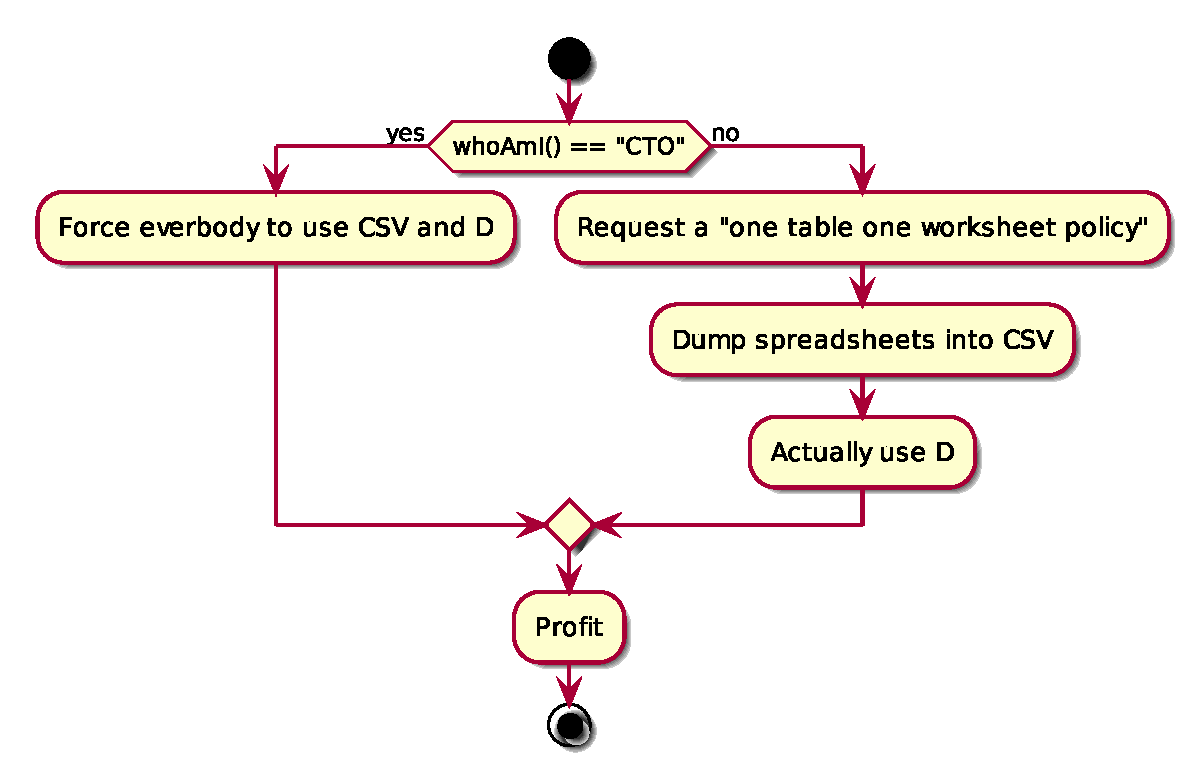
\includegraphics[width=0.8\textwidth]{attackvectors.eps}
		\end{center}
	\end{frame}

	\begin{frame}{Leveraging existing libraries}
		Writing data to spreadsheets
		\begin{itemize}
			\item Is is required, people will ask for that
			\item Writing a somewhat feature complete xlsx writer is a huge task
		\end{itemize}
		\mbox{}\\[1cm]
		\begin{itemize}
			\item libxlsxwriter is a feature (complete) xlsx writer
			\item Wrapping it by hand, no way (+78000 lines of structs, enums and functions)
			\item dpp to the rescue
			\item libxlsxwriter.d (+4000 lines)
			\item But it is still a C api
		\end{itemize}
	\end{frame}

	\begin{frame}[fragile]{Code example}
		\begin{lstlisting}[language=D]
void chart_axis_set_name(lxw_chart_axis*, const(char)*)
void chart_axis_set_name_range(lxw_chart_axis*, const(char)*, lxw_row_t, lxw_col_t)
void chart_axis_set_name_font(lxw_chart_axis*, lxw_chart_font*)
void chart_axis_set_num_font(lxw_chart_axis*, lxw_chart_font*)
void chart_axis_set_num_format(lxw_chart_axis*, const(char)*)
void chart_axis_set_line(lxw_chart_axis*, lxw_chart_line*)
void chart_axis_set_fill(lxw_chart_axis*, lxw_chart_fill*)
void chart_axis_set_pattern(lxw_chart_axis*, lxw_chart_pattern*)
void chart_axis_set_reverse(lxw_chart_axis*)
void chart_axis_set_crossing(lxw_chart_axis*, double)
void chart_axis_set_crossing_max(lxw_chart_axis*)
void chart_axis_off(lxw_chart_axis*)
		\end{lstlisting}
	\end{frame}

	\begin{frame}[fragile]{Code example}
		\begin{lstlisting}[language=D]
struct ChartAxis {
	lxw_chart_axis* handle;

	void setName(string name) { 
		chart_axis_set_name(this.handle, toStringz(name)); 
	}

	void setNameRange(string name, lxw_row_t row, 
			lxw_col_t col) 
	{
		chart_axis_set_name(this.handle, toStringz(name), row, col
			);
	}
	...
}
		\end{lstlisting}
	\end{frame}

\end{document}
